%%%%%%%%%%%%%%%%%%%%%%%%%%%%%%%%%%%%%%%%%%%%%%%%%%%%%%%
%                File: jonxml.tex                     %
%                     VERSION: 1.0                    %
%                Date: February 24, 2003              %
%                                                     %
%           LaTeX template file for use with          %
%        OSA's Journal of Optical Networking (JON)    %
%                                                     %
%  send comments to Scott Dineen, sdinee@osa.org      %
%                                                     %
% This file requires style file, jonxml.sty, under    %
%              the LaTeX article class                %
%                                                     %
%         \documentclass[10pt,letterpaper]{article}   %
%         \usepackage{jonxml}                         %
%                                                     %
%       (c) 2003 Optical Society of America           %
%%%%%%%%%%%%%%%%%%%%%%%%%%%%%%%%%%%%%%%%%%%%%%%%%%%%%%%

%% This new template for the Journal of Optical Network is
%% designed to assist conversion to XML

%%%%%%%%%%%%%%%%%%%%%%% preamble %%%%%%%%%%%%%%%%%%%%%%

\documentclass[10pt,letterpaper]{article}
\usepackage{jonxml}
\usepackage{hyperref}

%%%%%%%%%%%%%%%%%%%%%%% begin %%%%%%%%%%%%%%%%%%%%%%%%%%

\begin{document}

%%%%%%%%%%%%%%%%%% title page information %%%%%%%%%%%%%%

\title{\LaTeX{} template for authors submitting to the \textit{Journal of Optical Networking}}

\author{M. Scott Dineen and Alexine Moore}

\address{Publications Department, Optical Society of America, Washington, D.C., 20036}

\email{jon@osa.org} %% email address is required

% \homepage{http:...} %% author's URL, if desired

%%%%%%%%%%%%%%%%%%% abstract and OCIS codes %%%%%%%%%%%%%%%
%% [use \begin*{abstract}...\end{abstract} if exempt from copyright]

\begin{abstract}A basic LaTeX template and style file are provided for the \textit{Journal of Optical Networking} (JON). The new template and instructions are designed to assist conversion to XML. For information on purely style matters, see the JON style manual, \mbox{\url{http://www.osa-jon.org/submission}}. \end{abstract}

\ocis{000.0000, 999.9999.}% REPLACE WITH CORRECT OCIS CODES FOR YOUR ARTICLE

%%%%%%%%%%%%%%%%%%%%%%%%%%  body  %%%%%%%%%%%%%%%%%%%%%%%%%%

\section{Introduction}
To speed review and production, JON LaTeX articles should follow these guidlines:

\begin{description}

\item[(a) Math:] To help with conversion to MathML, place all math in a proper math environment. For example, expression $3\times 4 = 12$ should be set this way, \texttt{\$3$\backslash$times 4=12\$}, not this way, \texttt{3 \$$\backslash$times\$4=12}.

\item[(b) Markup:] Keep markup as simple as possible. Special spacing commands such as \texttt{$\backslash$,} and \texttt{$\sim$} should not be used, since they may complicate whitespace handling in the XML file.

\item[(c) Reference callouts:] Set reference callouts with standard \verb+\cite{}+ command or set manually inside square brackets (JON no longer uses superscript reference callouts \cite{IEEE98,Zhao02} or the \texttt{overcite} package). For more on references, see note \cite{refs} below.


\item[(d) Style:] Review and adhere to guidelines given in the \mbox{\href{http://www.osa-jon.org/submission}{JON style manual}}.

\end{description}

\section{Figures, Tables, and Multimedia}
JON encourages authors to submit color and multimedia figures with their manuscripts. Guidelines on multimedia submissions can be found at \mbox{\url{http://www.osa-jon.org/submission}}. Figures and tables may be placed in the body of the manuscript. To include multimedia, set a static image (e.g., frame from a video) in the manuscript as a figure, and upload multimedia files separately.


 \begin{table}[htb]
 \centering \textbf{\caption{Sample Table}}
\begin{tabular}{ccc}
    \hline
    One & Two & Three \\
    \hline
    Eins & Zwei & Drei \\
    Un & Deux & Trois \\
    Jeden & Dv\v{e} & T\v{r}i \\
    \hline
   \end{tabular}
    \end{table}

\begin{figure}[htb]
\centerline{\scalebox{.92}{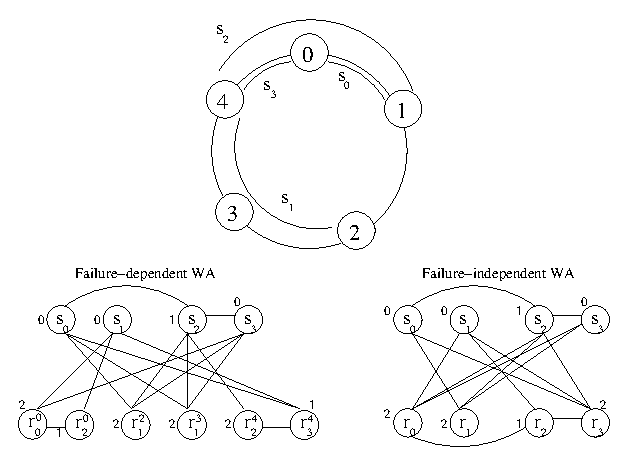
\includegraphics{JONF1.eps}}}

\caption{Sample caption (Ref. \cite{Sahin02}, Fig. 1).}
\end{figure}

\section{Conclusion}
After proofreading the manuscript, tar and gzip the \texttt{.tex} file and
figures; then enter the requested information into the JON
online submission system at \\
\url{http://www.osa-jon.org} and upload the tarred and gzipped
archive. If there is video or other multimedia, the associated
files should be uploaded separately.

All papers are accepted subject to editing to ensure readability
and conformity to journal style. Authors will receive page proofs
of their papers. Corrected proofs should be returned within 48
hours of receipt to avoid publication delays. For further
instructions, please see the JON web pages.


%\appendix
%\section*{Appendix A:  \LaTeX{} Code for Appendices}
%\setcounter{equation}{0}
%\renewcommand{\theequation}{A{\arabic{equation}}}

%acknowledgments
%\section*{Acknowledgments}

%%%%%%%%%%%%%%%%%%%%%%% References %%%%%%%%%%%%%%%%%%%%%%%

\begin{thebibliography}{99}
\bibitem{IEEE98} IEEE Standard 802.1Q-1998, ``IEEE standards for local and metropolitan area networks: virtual bridged local area networks'' (Institute of
Electrical and Electronics Engineers, New York, 1999), \url{http://www.ieee.org}.

\bibitem{Zhao02}  M. Zhao, G. Morthier, and R. Baets, ``Quasi-ideal optical decision characteristic from a Mach�Zehnder interferometer with gain-clamped semiconductor optical amplifiers,'' in \emph{Optical Fiber Communication Conference (OFC 2002)}, Vol. 70 of OSA Trends in Optics and Photonics Series (Optical Society of America, Washington, D.C., 2002), ThGG94, pp. 745--746.

\bibitem{refs} Please do not send separate Bib\TeX{} files. If you use Bib\TeX{}, you can simply paste the output (e.g., contents of \texttt{.bbl} file) into the bibliography section of the \texttt{.tex} file.

\bibitem{Sahin02} G. Sahin and M. Azizoglu, ``Wavelength-assignment algorithms for service and restoration in wavelength-division-multiplexing rings,'' J. Opt. Netw. {\bf 1,} 102--111 (2002), \url{http://www.osa-jon.org/abstract.cfm?URI=JON-1-2-102}.

\end{thebibliography}

%% use \url{} or \href for web links, with hyperref.sty
%%%%%%%%%%%%%%%%%%%%%%%%%%% end %%%%%%%%%%%%%%%%%%%%%%%%%%%

\end{document}
